\documentclass[../main.tex]{subfiles}
\begin{document}
\subsection{Chow rings}
\begin{example}[Chow ring of $\overline{\mathrm{M}}_{0,n}$]
Let's start with $\overline{\mathrm{M}}_{0,4}\cong \mathbb{P}^{1}$, then we have $\delta_{1,2}=\delta_{1,3}=\delta_{1,4}$, and $\delta_{1,2}\delta_{1,3}=0$. We get the Chow ring 
$$\mathrm{CH}^{*}(\mathbb{P}^{1})\cong \mathbb{Z}[\delta]/(\delta^{2}).$$
How about $\overline{\mathrm{M}}_{0,5}$? We have $\binom{5}{2}=10$ generators $\delta_{i,j}$ with the relations
\begin{itemize}
\item For distinct i,j,k,l
$$\delta_{i,j}+\delta_{k,l}=\delta_{i,k}+\delta_{j,l}=\delta_{i,l}+\delta_{j,k}$$
\item multiply the equations above by $\delta_{i,j}$, and apply the third relation in Keel's description, we get double products 
$$\delta_{i,j}^{2}=\delta_{k,l}^{2}=-\delta_{a,b}\delta_{c,d}$$
\item all triple products and above vanish by dimensional argument.
where $a,b,c,d$ are any $4$ distinct elements in $\{1,2,3,4,5\}$.
\end{itemize}
Well, what is this ring exactly? Let's do more trivial computations, if we label $\{\delta_{1,2},\delta_{1,3},\dots ,\delta_{2,3},\dots , \delta_{4,5}\}$ lexicographically as $\{e_{1},\dots, e_{10}\}$, the only complicated part of $\mathrm{CH}^{*}(\overline{\mathrm{M}}_{0,5})$ is the $\mathrm{Pic}(\overline{\mathrm{M}}_{0,5})$, use the first relation above, it's given by the cokernel of the matrix in the first figure below.
\begin{figure}[h!]
\centering
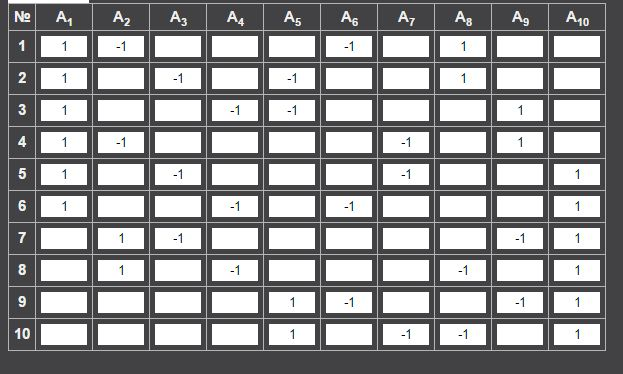
\includegraphics[width=\textwidth]{img/matrix.JPG}
\caption{Linear relations among $\delta_{i,j}$}
\label{Linear relations among boundary divisors}
\end{figure}
Carry out the standard elimination algorithm, we get the matrix in the second figure below,
\begin{figure}[h!]
\centering
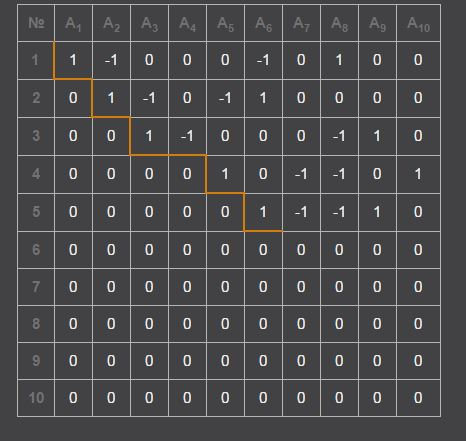
\includegraphics[width=\textwidth]{img/matrix2.JPG}
\caption{Linear relations among $\delta_{i,j}$}
\label{Linear relations among boundary divisors}
\end{figure}
this tells us that 
$$\mathrm{rank}(\mathrm{Pic})(\overline{M}_{0,5})=5$$
To be more precise, we have 
$$\delta_{1,2}=\delta_{1,3}+\delta_{2,4}-\delta_{3,4}$$
$$\delta_{1,3}=\delta_{1,4}+\delta_{2,3}-\delta_{2,4}$$
$$\delta_{1,4}=\delta_{1,5}+\delta_{3,4}-\delta_{3,5}$$
$$\delta_{2,3}=\delta_{2,5}+\delta_{3,4}-\delta_{4,5}$$
$$\delta_{2,4}=\delta_{2,5}+\delta_{3,4}-\delta_{3,5}$$
$$\delta_{1,5}, \delta_{2,5},\delta_{3,4},\delta_{3,5},\delta_{4,5}\text{ are free generators}$$
These computations tell us, Keel's description of $\mathrm{CH}^{*}(\overline{M}_{0,n})$ is not necessarily an easy and clean one. On the other hand, we can give a more geometric description of the computation of $\mathrm{CH}^{*}(\overline{\mathrm{M}}_{0,5})$ here by realizing $\mathrm{CH}^{*}(\overline{\mathrm{M}}_{0,5})$ as a blow-up of $\mathbb{P}^{1}\times \mathbb{P}^{1}$ along $3$ distinct points on the diagonal. That is the universal curve diagram 

$$\begin{tikzcd}
\mathscr{U}_{g,n+1}\arrow{rr}{\text{contraction}}\arrow{d}{\pi_{n+1}}& & \mathscr{U}_{g,n}\times_{\overline{\mathrm{M}}_{g,n}}\mathscr{U}_{g,n}\arrow{r}\arrow{d} & \mathscr{U}_{g,n}\arrow{d}{\pi_{n}}\\
\overline{\mathrm{M}}_{g,n+1}\arrow{rr}{\cong}& &\mathscr{U}_{g,n}\arrow{r}{\pi_{n}} & \overline{\mathrm{M}}_{g,n}
\end{tikzcd}$$
specializes to 
$$
\begin{tikzcd}
\overline{\mathrm{M}}_{0,5}\cong Bl_{(0,0),(1,1),(\infty, \infty)}(\mathbb{P}^{1}\times \mathbb{P}^{1})\arrow{rr}{\text{contraction}}\arrow{d}{\pi_{4}}& & \mathbb{P}^{1}\times \mathbb{P}^{1}\arrow{r}\arrow{d} & \mathbb{P}^{1}\arrow{d}{\pi_{3}}\\
\overline{\mathrm{M}}_{0,4}\arrow{rr}{\cong}& &\mathbb{P}^{1}\arrow{r}{\pi_{3}} & \overline{\mathrm{M}}_{0,3}\cong pt
\end{tikzcd}$$
The blow-up of $\mathbb{P}^{2}$ at two points is isomorphic to the blow-up of $\mathbb{P}^{1}\times \mathbb{P}^{1}$ at one point. To see this,  think about the geometry here $Bl_{2pts}(\mathbb{P}^{2})$ contains three $(-1)$-divisors, namely, $E_{1}, E_{2}$ and $H-E_{1}-E_{2}$(the strict transformation of the line passing the two points). If we blow down the divisor $H-E_{1}-E_{2}$, Consider the ample divisor $2H-E_{1}-E_{2}$, this corresponding to conics passing the two points, we get a degree $2$ smooth surface in $\mathbb{P}^{3}$, 
over an algebraically closed field, it's isomorphic to $\mathbb{P}^{1}\times \mathbb{P}^{1}$ which just contracts the strict transformation of the line passing through the two points. Then we know $\overline{\mathrm{M}}_{0,5}\cong Bl_{4pts}(\mathbb{P}^{2})$, the Chow ring structure is given by 
$$\mathrm{CH}^{*}(\overline{\mathrm{M}}_{0,5})\cong \mathbb{Z}[H, E_{1},E_{2}, E_{3}, E_{4}]/(H^{2}-1, HE_{i}, E_{i}^{2}+1, E_{i}E_{j}).$$
Finally, we want to ask, what are those $\delta_{i,j}$'s in this ring?
\end{example}
\begin{remark}[Keel, Chow ring of $\overline{\mathrm{M}}_{0,n}$]
Sean Keel computed $\mathrm{CH}^{*}(\overline{\mathrm{M}}_{0,n})$ in the paper \href{http://www.math.colostate.edu/~renzo/teaching/Topics10/keel.pdf}{Intersection theory of moduli space of stable $n$-pointed curves of genus $0$}. Which says that $\mathrm{CH}^{*}(\overline{\mathrm{M}}_{0,n})$ is generated by boundary divisors $\{\delta_{S}|S\subset \{1,2,\dots, n\}, \#S \geq2, \# S^{c}\geq2\}$ subject to the following relations
\begin{itemize}
\item $\delta_{S}=\delta_{S^{c}}$.
\item For any distinct $i,j,k,l\in \{1,2,\dots, n\}$ 
$$\sum_{i,j\in S, k,l\in S^{c}}\delta_{s}=\sum_{i,k\in S, k,l\in S^{c}}\delta_{s}=\sum_{i,l\in S, j,k\in S^{c}}\delta_{s}$$
\item $\delta_{S}\delta_{T}=0$ unless $S\subset T, S\subset T^{c}, S^{c}\subset T, S^{c}\subset T^{c}$.
\end{itemize}
\end{remark}
\begin{remark}[Blow-ups of $\mathbb{P}^{2}$]
Here, we have to be a little bit careful. We know $Bl_{2pts}(\mathbb{P}^{2})$ is isomorphic to $Bl_{pt}(\mathbb{P}^{1}\times \mathbb{P}^{1})$, but note that $\mathbb{F}_{1}\cong Bl_{pt}(\mathbb{P}^{2})\ncong \mathbb{P}^{1}\times \mathbb{P}^{1}$ because on $\mathbb{P}^{1}\times \mathbb{P}^{1}$ we don't have any $(-1)$-curve! This fact also tells us that $\mathbb{F}_{1}:=\mathbb{P}(\mathcal{O}\oplus\mathcal{O}(1))$ is not minimal, all other $\mathbb{F}_{n}$'s are minimal! To conclude,
\begin{itemize}
\item $Bl_{\text{$3$ distinct points on $\Delta$}}(\mathbb{P}^{1}\times \mathbb{P}^{1})\cong Bl_{\text{$4$ general points }}(\mathbb{P}^{2})$
\item $Bl_{\text{$3$ general points}}(\mathbb{P}^{1}\times \mathbb{P}^{1})\cong Bl_{\text{$3$ distinct points on $\Delta$}}(\mathbb{P}^{1}\times \mathbb{P}^{1})$
\item $Bl_{\text{$4$ general points }}(\mathbb{P}^{2})\ncong Bl_{\text{4pts, 3 on a line}}(\mathbb{P}^{2})$
\item If we blow-up three  points on a line $L$ in $\mathbb{P}^{2}$, the total transformation $L'$ of the $L$ is in the class $H-E_{1}-E_{2}-E_{3}$, thus $L'^{2}=-2$, thus we get a $(-2)$-curve, the ordinary blow-up doesn't have any $(-2)$-curve. 

\end{itemize}
\end{remark}




%%%%%%%%%%%%%%%%%%%%%%%%%%%%%%%%%%%%
\subsection{Five conics problems via fundamental class}
Excess intersection theory or intersection theory on the space of complete conics (i.e Blow up of the degree $2$ Veronese surface in $\P(\H^{0}(\O_{\P^{2}}(2)))\cong \P^{5}$) shows that $3264$ smooth conics tangent to $5$ generic conics. Here we want to interpret the the computations in excess intersection theory in term of the construction of the fundamental class of a moduli problem. We know the locus of conics that are tangent to a given conic is a degree $6$ hypersurface in $\P^{5}$. We have to consider the intersection $\M=\bigcap_{i=1}^{5}Z_{i}$ degree $6$ hypersurfaces of this form, each with defining equation $f_{i}$. We view them as sections of $\O_{\P^{5}}(6)$. The universal property of $\M$ comes from the fact that it's a fibre product. $\M$ is not a complete intersection, the construction of the fundamental class in this case is just that we scaling the images all those global sections $f_{i}\rightarrow tf_{i}$. When $t\rightarrow +\infty$, we end up with the normal cone $C_{\M/\P^{5}}$ of $\M$ in $\P^{5}$, which lives in $E:=\bigoplus_{i=1}^{5}\O_{\P^{5}}(6)$, and the support of it is just $\M$.  Although the cone is not a global section of $E|_{\M}$. The principle of fundamental classes is just that we view it as a global section. Then $[\M]^{\vir}$ is defined to be $[C_{\M}/\P^{5}|_{\M}]\cap \M$, this intersection is well-defined because we have the Gysin isomorphism $0^{!}: A_{k}(E)\rightarrow A_{k-\mathrm{rk}{E}}(\M)$. In other words, we're in the following situation.
$$
\begin{tikzcd}
C_{\M/\P^{5}}|_{\M}\arrow{r}\arrow{d} & E=\O^{\oplus 5}_{\P^{5}}(6)\arrow{d}\\
\M\arrow{r} &\P^{5}
\end{tikzcd}
$$
The computation of $[\M]^{\vir}$ boils down to the computation of the Gysin map. To do it, we have
$$\begin{tikzcd}
\M\arrow[d, equal]\arrow{r}{\text{c.l}} & C_{\M}/\P^{5}|_{\M}\arrow{d}{\text{c.l}}\\
\M \arrow{r}{\text{c.l}} & E|_{\M}
\end{tikzcd}
$$
Where `c.l' stands for closed embedding. In this situation, we have (see for example Ravi Vakil's notes \href{http://math.stanford.edu/~vakil/245/245class16.pdf}{here}) 
$$[C_{\M/\P^{5}}|_{\M}]\cap [\M]=\{c(E|_{\M})s(\M, C_{\M/\P^{5}}|_{\M})\}_{0}.$$
The normal cone is just the normal bundle, but one subtle thing here is that although set-theoretically the $2$ dimensional component $T$ of $\M$ is just the degree $2$ Veronese surface $S$, scheme-theoretically, it's not. The multiplicity of $Z_{i}$ along $S$ is $2$ (see for example Eisenbud's book \href{https://scholar.harvard.edu/files/joeharris/files/000-final-3264.pdf}{here}, p463). Then we know the degree $k$ piece of the segre class $s(\M, C_{\M/\P^{5}}|_{\M})$ is given by 
$$s_{k}(\M, C_{\M/\P^{5}}|_{\M})=2^{k+3}s(S, N_{S/\P^{5}})+s_{k}(\text{zero dimensional components of $\M$}).$$
Now we compute 
$$c(E|_{\M})=(1+6H)^{5}|_{\M}=(1+12h)^{5}.$$
$$c(N_{S/\P^{5}})=\frac{(1+H)^{6}|_{S}}{(1+h)^{3}}=1+9h+30h^{2}.$$
Which implies
$$s(S, N_{S/\P^{5}})=1-9h+51h^{2}.$$
Thus
$$s_{k}(\M, C_{\M/\P^{5}}|_{\M})=8-144h+1632h^{2}+s_{k}(\text{zero dimensional components of $\M$}).$$
Finally, we get 
$$[\M]^{\vir}=\deg((1+12h)^{5}(8-144h+1632h^{2}))+\text{zero dimensional components of $\M$}$$
$$=4512[\text{pt on $T$}]+\text{zero dimensional components of $\M$}.$$
Now use the fact that $$i_{*}[\M]^{\vir}=c_{\mathrm{top}}(E)=7776[\text{pt on $\P^{5}$}]$$
We get 
$$\text{number of zero dimensional components of $\M$}=7776-4512=3264.$$
However, from the point of view of fundamental classes, the important thing is not the solution $3264$ of the five conics problem, it's the fact that $[\M]^{\vir}$ is given by $4512$ points on the non-reduced Veronese surface plus all zero dimensional components of $\M$.
\subsection{Quantum cohomology of projective spaces} We apply basic Schubert calculus to prove that 
$$QH^{*}(\P^{n}, \Z)=\Z[h_{1},q]/(h_{1}^{n+1}-q).$$
The most annoying part is the notation, we use the following
$$
\begin{tabular}{ |p{3cm}||p{3cm}|p{3cm}|p{3cm}|  }
 \hline
 \multicolumn{4}{|c|}{$\P^{n}$} \\
 \hline
 \text{Algebraic cycles}& $\H_{*}(\P^{n}, \Z)$ & $\H^{*}(\P^{n},\Z)$ &\text{Differential forms}\\
 \hline
 \text{[pt]}  & $\H_{0}, H^{n}$    & $\H^{0}, h_{0}$ &  \text{constant functions}\\
 \hline
  \text{[$\P^{1}$]}  & $\H_{2}, H^{n-1}$    & $\H^{2}, h_{1}$ &  \text{$(1,1)$-forms}\\
 \hline
 ...&...&...&...\\
 \hline
   \text{[$\P^{n}$]}  & $\H_{2n}, H^{0}$    & $\H^{2n}, h_{n}$ &  \text{$(n,n)$-forms}\\
 \hline
\end{tabular}
$$
Two extra terms for the computation
$$\H_{2}(\P^{n}, \Z)=\Z H^{n-1}, q^{rH^{n-1}}\leftrightarrow q^{r}$$
$$\dim \M_{0,3}(\P^{n}, rH^{n-1})=(\dim \P^{n}-3)(1-0)+3+\int_{rH^{n-1}}T_{\P^{n}}=n+r(n+1).$$
The quantum product is defined to be 
$$h_{i}\circ h_{j}:=\sum (h_{i}\circ h_{j})_{rH^{n-1}}q^{r}$$
$$=\sum\langle H^{i}|H^{j}|H^{k}\rangle_{rH^{n-1}}h_{k}q^{r}.$$
Since $\ev_{1}^{*}(H^{i})\cup \ev_{2}^{*}(H^{j})\cup \ev^{*}_{3}(H^{k})$ cuts down the dimension of $\M_{0,3}(\P^{n}, rH^{n-1})$ by at most $3n$. Thus $\langle H^{i}|H^{j}|H^{k}\rangle_{rH^{n-1}}\neq 0$ only if $r=0$ or $1$. First we have the classical intersection part 
$$\langle H^{i}|H^{j}|H^{k}\rangle_{0}=\begin{cases}1 & i+j+k=n\\
0 & \text{otherwise}.\end{cases}$$
To compute $\langle H^{i}|H^{j}|H^{k}\rangle_{1H^{n-1}}$, we use basic Schubert calculus. The geometric meaning of  $\langle H^{i}|H^{j}|H^{k}\rangle_{1H^{n-1}}$ is that projective lines intersecting with $H^{i}, H^{j}$ and $H^{k}$. In other words, it means $2$-planes in $\C^{n+1}$ intersecting $(n+1-i)$-plane, $(n+1-j)$-plane and $(n+1-k)$-plane nontrivially. In $\Gr(2, n+1)$, the Schubert cycle corresponding to $2$-planes intersecting a $l$-plane nontrivially is exactly $\sigma_{n+1-2-l+1}$. Thus we have to compute 
$$\sigma_{i-1}\sigma_{j-1}\sigma_{k-1}\in A^{*}(\Gr(2, n+1)).$$
Luckily, they're all special cycles in the sense that we can apply Pieri's rule. Note that the quantum product only takes the degree $0$ part. Now the question is that how many different ways can we find to add $(j-1)+(k-1)$ boxes (in different columns) to a length $i-1$ row such that we can finally fill up a $2(n-1)$-rectangular? The only possibility is that $(i-1)+(j-1)+(k-1)=2n-2$, that is $i+j+k=2n+1$. And in this case, we have exactly a unique way to fill up the rectangular. In conclusion, we have 
$$\langle H^{i}|H^{j}|H^{k}\rangle_{H^{n-1}}=\begin{cases}1 & i+j+k=2n+1\\
0 & \text{otherwise}.\end{cases}$$
All together, we get the desired 
$$QH^{*}(\P^{n}, \Z)=\Z[h_{1},q]/(h_{1}^{n+1}-q).$$
\subsection{Quantum cohomology of the flag variety associated to a unitary group}
Consider the flag variety 
$$F_{3}=F_{1,2}=\{(L,V)\in \Gr(1, \C^{3})\times \Gr(2,\C^{3})|L\subset V\}\cong U_{3}/(U_{1}\times U_{1}\times U_{1}).$$
We have 
$$QH^{*}(\P(\mathcal{V})), \Z)=\Z[\alpha, \zeta]/(\zeta^{2}-\alpha\zeta+\alpha^{2}-q_{1}-q_{2}, \alpha^{3}-\alpha q_{1}-\zeta q_{1}).$$
First note that $F_{3}$ is nothing but the projectivization of the tautological bundle $\mathcal{V}$ on $\Gr(2, \C^{3})$. We denote it by $\P(\mathcal{V})$. Since the Schubert cells give $\P(\mathcal{V})$ a CW-structure, the cohomology ring is the same as the Chow ring. Let $\zeta=c_{1}(\O_{\P(\mathcal{V})}(1))$, then $$A^{*}(\P(\mathcal{V}))=A^{*}(\Gr(1, \C^{3}))[\zeta]/(\zeta^{2}+c_{1}(\mathcal{V})\zeta+c_{2}(\mathcal{V})).$$
$$c(\mathcal{V})=1-\sigma_{1}+\sigma_{1,1}=1-[\P^{1}]+[pt].$$
We have the following 
$$
\begin{tabular}{ |p{3cm}||p{3cm}|p{3cm}|p{5cm}|  }
 \hline
 \multicolumn{4}{|c|}{$\P(\mathcal{V})$} \\
 \hline
 \text{Algebraic cycles}& $\H_{*}(\P(\mathcal{V}), \Z)$ & $A^{*}(\P(\mathcal{V}),\Z)$ &\text{Algebraic cocycles}\\
 \hline
 \text{[pt]}  & $\H_{0}$    & $\H^{0}; 1$ & $[\P(\mathcal{V})]$\\
 \hline
  \text{$\pi^{*}[pt]$}, \text{$[\P^{1}]$}  & $\H_{2}; F, L $    & $\H^{2}; \zeta, \alpha$ & $[\P^{2}], \pi^{*}[\P^{1}]$\\
 \hline
 \text{$\pi^{*}[\P^{1}]$},$[\P^{2}]$ & $\H_{4}; l,f$    & $\H^{4}; \alpha^{2}, \zeta^{2}$ &  $\pi^{*}[pt]=[\text{Fibre}], [\P^{1}]$\\
 \hline
   \text{[$\P(\mathcal{V})$]}  & $\H_{6}$    & $\H^{6};\alpha^{2}\zeta= \alpha\zeta^{2} $ &  $[\text{pt}]$\\
 \hline
\end{tabular}
$$
Here by `algebraic cocycles', we just mean algebraic cycles graded by their codimensions. Here we give different names to the same algebraic cycle depends on we view it as elements in $\H^{*}$ or $\H_{*}$. In this notation, we rewrite 
$$A^{*}(\P(\mathcal{V}))=\Z[\alpha,\zeta]/(\zeta^{2}-\alpha\zeta+\alpha^{2}, \alpha^{3}).$$
Two extra terms we need for the computation of the quantum cohomology ring 
$$\H_{2}(\P(\mathcal{V}), \Z)=\Z F\oplus \Z L, q^{rF+sL}\leftrightarrow q_{1}^{r}q_{2}^{s}$$
$$\dim \M_{0,3}(\P(\mathcal{V}), rF+sL)=(\dim \P(\mathcal{V})-3)(1-0)+3+\int_{rF+sL}c_{1}(T_{\P(\mathcal{V})})=3+2r+2s.$$
Here we used the fact that $c_{1}(T_{\P(\mathcal{V})})=2\zeta+2\alpha$.
As an example, we compute $\alpha\circ \alpha$
\begin{align*}
\alpha\circ \alpha :&=\sum (\alpha\circ \alpha)_{rF+sL}q_{1}^{r}q_{2}^{s} \\
&=\sum_{(r,s)}\sum_{\gamma\in \H_{*}}\langle l|l|\gamma\rangle_{rF+sL}\gamma^{\vee}q_{1}^{r}q_{2}^{s}.
\end{align*}
Now we compute
\begin{align*}
\langle l,l,l\rangle_{(0,0)} &= l^{3}=\alpha^{3}=0, \\
\langle l,l,f\rangle_{(0,0)} &= \alpha^{2}\zeta=[pt], \deg([pt])=1.
\end{align*}
$$f^{\vee}=\alpha^{2}.$$
Similarly,
\begin{align*}
\langle l|l|[pt]\rangle_{(1,0)} &= F, \\
\langle l|l|[pt]\rangle_{(0,1)} &= \Gr(1, \P^{2}).
\end{align*}
Then we know there's exactly one stable map of degree $1$ intersecting two different $l$. But the moduli space of degree $1$ stable maps to the base $\P^{2}$  has positive dimension, which gives us Gromov-Witten invariant $0$. In other words, we have 
$$\alpha\circ \alpha =f^{\vee}+1q^{1}=\alpha^{2}+q_{1}.$$
Similar argument gives us
$$\zeta\circ \zeta=\zeta^{2}+q_{2}$$
Then we finally get the quantum cohomology ring of $\P(\mathcal{V})$
$$QH^{*}(\P(\mathcal{V})), \Z)=\Z[\alpha, \zeta]/(\zeta^{2}-\alpha\zeta+\alpha^{2}-q_{1}-q_{2}, \alpha^{3}-\alpha q_{1}-\zeta q_{1}).$$
In Martin A. Guest's book \href{http://www.f.waseda.jp/martin/preprints/qcis-preprint.pdf}{`From cohomology to integrable systems', Example 2.6}, you can find another computation of this quantum cohomology ring, the result is given by
$$QH^{*}(\P(\mathcal{V}), \Z)=\frac{\Z[x_{1}, x_{2}, x_{3}, q_{1}, q_{2}, q_{3}]}{(x_{1}+x_{2}+x_{3}, x_{1}x_{2}+x_{1}x_{3}+x_{2}x_{3}+q_{1}+q_{2}+q_{3}, x_{1}x_{2}x_{3}+x_{1}q_{2}+x_{3}q_{1})}.$$
And
$$QH^{*}(\P(\mathcal{V}), \Z)=\Z[a,b, q_{1}, q_{2}]/(a^{2}+b^{2}-ab-q_{1}-q_{2}, ab^{2}-a^{2}b-aq_{2}-bq_{1}).$$
Our result is easily seen to be the same as the second one because 
$$\alpha(\zeta^{2}-\alpha\zeta+\alpha^{2}-q_{1}-q_{2})-(\alpha^{3}-\alpha q_{1}-\zeta q_{1})=\alpha\zeta^{2}-\alpha^{2}\zeta-\alpha q_{2}+\zeta q_{1}.$$
\subsection{Examples of quantum differential equations}
\subsection{Equivariant cohomology}
We view equivariant cohomology as the geometry of a system of varieties and view equivariant Chern classes as information contained in a system of vector bundles. We'll show this with some examples. By the approximation theorem in equivariant cohomology, we know if $\mathbb{E}_{m}$ is a connected space with a free $G$-action and $H^{i}(\mathbb{E}_{m})=0$ for $0<i<k(m)$, then 
$$\H_{G}^{*}(X):=\H^{*}(\mathbb{E}G\times_{G}X)=\H^{*}(\mathbb{E}_{m}\times_{G}X), \forall *<k(m).$$
\begin{example}[$G=(\C^{\times})^{n}, X=\mathrm{pt}$]
Our point here is that we can think about the basic result $\H^{*}(\mathrm{pt})=\Z[t_{1}, \dots, t_{n}]$ as taking the cohomology of the chain of varieties
$$
\begin{tikzcd}
\mathrm{pt}\arrow[equal]{d} \arrow[hookrightarrow]{r} 
  & \mathrm{pt}\times_{G}(\C^{1}\setminus\{0\})^{n}\arrow[hookrightarrow]{r}\arrow[equal]{d} 
  & \dots \arrow[hookrightarrow]{r}\arrow[equal]{d} 
  & \mathrm{pt}\times_{G}(\C^{m}\setminus\{0\})^{n}\arrow[hookrightarrow]{r}\arrow[equal]{d}
  & \dots \\
\mathrm{pt} \arrow[hookrightarrow]{r} 
  & (\P^{1})^{n}\arrow[hookrightarrow]{r} 
  & \dots\arrow[hookrightarrow]{r}
  & (\P^{m-1})^{n}\arrow[hookrightarrow]{r}
  & \dots 
\end{tikzcd}
$$
We can also view it in the usual way, that is $\H^{*}_{G}(\mathrm{pt})=\H^{*}((\P^{\infty})^{n})$.
\end{example}
\begin{example}[$G=(\C^{\times})^{n}, X=\Gr(k,n)$]
As we indicated, $\H^{*}_{G}(\Gr(k,n))$ is given by the chain of varieties $\Gr(k,n)\times_{G}(\C^{m}\setminus\{0\})^{n}$. We shall show it's just a sequence of Grassmannian bundles over products of projective spaces.
$$
\begin{tikzcd}
\Gr(k,n)\arrow{d} \arrow[hookrightarrow]{r} 
  & \Gr(k,n)\times_{G}(\C^{1}\setminus\{0\})^{n}\arrow[hookrightarrow]{r}\arrow{d} 
  & \dots \arrow[hookrightarrow]{r}\arrow{d} 
  & \Gr(k,n)\times_{G}(\C^{m}\setminus\{0\})^{n}\arrow[hookrightarrow]{r}\arrow{d}
  & \dots \\
\mathrm{pt} \arrow[hookrightarrow]{r} 
  & (\P^{1})^{n}\arrow[hookrightarrow]{r} 
  & \dots\arrow[hookrightarrow]{r}
  & (\P^{m-1})^{n}\arrow[hookrightarrow]{r}
  & \dots \\
E\arrow{u} \arrow[hookrightarrow]{r} 
  & E\times_{G}(\C^{1}\setminus\{0\})^{n}\arrow[hookrightarrow]{r}\arrow{u} 
  & \dots \arrow[hookrightarrow]{r}\arrow{u} 
  & E\times_{G}(\C^{m}\setminus\{0\})^{n}\arrow[hookrightarrow]{r}\arrow{u}
  & \dots
\end{tikzcd}.
$$
Where $E=\C^{n}$ with the standard torus action. Then we know
$$V_{m}:=E\times_{G}(\C^{m}\setminus\{0\})^{n}=\oplus_{i=1}^{n}\O_{i}(-1).$$
This is is the fibres of $E$ has the same weights as the base. Naturally,
$$\Gr(k,n)\times_{G}(\C^{m}\setminus\{0\})^{n}=\Gr(V_{m},k).$$
In other words, it's just the Grassmannian bundle of $k$-planes associated to the vector bundle $V_{m}$. By knowledge of the cohomology of the Grassmannian bundle, we conclude that 
$$\H^{*}_{G}(\Gr(k,n))=\Z[t_{1}, \dots, t_{n}][c_{1}, \dots, c_{k},c'_{1}, \dots, c'_{n-k}]/((1+c_{1}+\dots+c_{k})(1+c_{1}'+\dots+c_{n-k}')=c(V)).$$
More precisely,
$$\H^{*}_{G}(\Gr(k,n))=\frac{\Z[t_{1}, \dots, t_{n}][c_{1}, \dots, c_{k},c'_{1}, \dots, c'_{n-k}]}{\{\frac{c(V)}{1-\sigma_{1}+\dots+(-1)^{k}\sigma_{k}}\}^{l}, \forall l>\dim(\Gr(V))-n+k}.$$
The denominator means that all terms with codimension as least $l+1$ vanish (actually, we only need the codimsion $l+1$ relation). As a special case, we get 
$$\H^{*}_{G}(\P^{n-1})=\Z[t_{1}, \dots, t_{n}][\zeta]/\prod_{i=1}^{n}(\zeta+t_{i}).$$
\end{example}
\begin{remark}[$\O(-1)$ or $\O(1)$ ?]
If the action on the fibres have the same weights as the base, then it's the tautological bundle (on $\P^{k}$ or Grassmannians). Tautological bundle has no global section, then we can tell it's $\O(-1)$. 
\end{remark}
\begin{remark}
\href{https://www.impan.pl/~pragacz/anderson1.pdf}{An introductory notes on equivariant cohomology here}
\end{remark}


\end{document}